\documentclass[NormeDiProgetto.tex]{subfiles}

\begin{document}
	
	\chapter{Processi di supporto}
	
	\section{Documentazione}
	\subsection{Descrizione}
	Questo capitolo descrive le scelte intraprese per la
	stesura, \citGloss{verifica} e approvazione riguardante la documentazione ufficiale.
	Tali norme sono tassative per tutti i documenti formali.
	Tali documenti sono elencati successivamente nella sotto-sezione "Documenti correnti". 
	
	\subsection{Ciclo di vita documentazione}
	Ogni documento formale deve passare gli stadi di "Sviluppo", "Verifica" e "Approvato".
	\begin{itemize}
		\item \textbf{Sviluppo:} inizia con la creazione del documento e termina con la conclusione della stesura di tutte le sue parti. In questa fase i Redattori aggiungono le parti assegnate tramite \citGloss{ticket}.
		Il passaggio alla fase di \citGloss{verifica} è automatizzato con la segnalazione al Responsabile;
		
		\item \textbf{Verifica:} il documento entra nella fase di verifica dopo l'assegnazione da parte del Responsabile. I Verificatori effettueranno le proc
		edure di controllo dello stesso.\\
		Al termine del controllo in caso positivo il documento entra automaticamente in fase di "Approvato", altrimenti i loro riscontri vengono consegnati al Responsabile di Progetto, che provvederà ad assegnare nuovamente il documento ad un Redattore attraverso una nuova fase di Sviluppo; 
		
		\item \textbf{Approvato:} l'approvazione di un documento coincide con il superamento positivo da parte di un verificatore dello stadio di \citGloss{verifica} comunicato al Responsabile che approva il documento per il rilascio esterno.
	\end{itemize}
	
	\subsection{Separazione documenti interni ed esterni}
	Ogni documento formale dovrà essere classificato come Interno
	oppure Esterno con le seguenti differenze:
	\begin{itemize}
		\item \textbf{Interno:} ha utilizzo interno al gruppo 353, redatto in lingua Italiana;
		\item \textbf{Esterno:} verrà condiviso con la Proponente ed i committenti, nel caso sia utile per il deploy dell'applicazione web o per il suo utilizzo da parte degli utenti finali, dovrà essere redatto in lingua Inglese.
	\end{itemize}
	Un documento formale farà sempre parte di una delle due categorie elencate.
	
	\subsection{Nomenclatura documenti}
	Tutti i documenti formali tranne Verbali e Lettera di Presentazione seguiranno questo sistema di nomenclatura:

	\begin{itemize}
		\item\textbf{ NomeDocumento:} indica il nome del documento senza spazi e lettere maiuscole all'inizio di ogni parola;
		\item \textbf{vX.Y.Z:} indica il numero di versionamento con X,Y e Z numeri interi e non negativi.	
	\end{itemize}
	Di seguito la spiegazione che assumono le versione del documento:
	\begin{itemize}
		\item \textbf{X:} rappresenta il numero di pubblicazioni ufficiali del documento: ogni qual volta il documento viene pubblicato il valore di Y e Z viene azzerato, quello di X incrementato di uno;
		\item \textbf{Y:} rappresenta il numero di verifiche completate con successo, in caso di mancato superamento della fase di \citGloss{verifica} il valore non va modificato, mentre se superata viene incrementato di uno e si azzera il valore della Z;
		\item \textbf{Z:} rappresenta il numero di modifiche effettuate al documento durante il suo sviluppo.	
	\end{itemize}
	Formato dei file: ogni documento si trova nel formato .tex durante il suo ciclo di vita.
	Dopo lo stato di “Approvato” per il documento viene quindi creato un \citGloss{PDF} contenente la versione approvata dal Responsabile.
	
	\subsection{Documenti correnti}
	Qui di seguito si presentano i documenti formali in ordine alfabetico, classificati per appartenenza (Interno ed Esterno):
	\begin{itemize}
		\item \textbf{Analisi dei Requisiti:} utilizzo Esterno, sigla (AR) \\
		 Documento per esporre e scomporre i \citGloss{requisiti} del progetto contenente casi d'uso relativi al prodotto e diagrammi di interazione con l'utente. Viene scritto dagli Analisti dopo aver analizzato il capitolato e interagendo con il Proponente in riunioni esterne;
		
		\item \textbf{Glossario:}
		utilizzo Esterno, sigla (GL) \\
		Documento per raccogliere le definizioni dei termini o concetti che saranno usati nei documenti formali per facilitarne la comprensione;
		
		\item \textbf{Norme di Progetto:}
		utilizzo Interno, sigla (NdP) \\
		Documento per mostrare le direttive e gli standard utilizzati all'interno del gruppo di lavoro 353
		per lo sviluppo del progetto;
		
		\item \textbf{Piano di Progetto:}
		utilizzo Esterno, sigla (PdP) \\
		Documento per l'analisi e la pianificazione della gestione delle risorse di tempo e umane;
		
		\item \textbf{Piano di Qualifica:}
		utilizzo Esterno, sigla (PdQ) \\
		Documento per descrivere standard e obiettivi che il gruppo dovrà raggiungere per garantire la qualità di prodotto e processo;
		
		\item \textbf{Studio di Fattibilità:}
		utilizzo Interno, sigla (SdF) \\
		Documento per indicare le riflessioni, punti di forza e caratteristiche sfavorevoli per ogni capitolato che ha portato alla scelta finale del gruppo.
		
	\end{itemize}
	
	\subsection{Norme}
	\subsubsection{Struttura dei documenti}
		Ogni documento è realizzato a partire da una disposizione prestabilita che dovrà essere conforme per ogni documento ufficiale ad eccezione dei verbali e della lettera di presentazione:
		\begin{itemize}
			\item \textbf{Frontespizio:} questa sezione si troverà nella prima pagina di ogni documento e conterrà:
			\begin{itemize}
				\item Logo del gruppo;
				\item Titolo del documento;
				\item Versione del documento con l'ultima data di modifica;
				\item Nome del gruppo;
				\item Nome del progetto.
			\end{itemize}
			
			\item \textbf{Informazioni sul documento:} conterrà la lista di responsabili,
			redattori, verificatori del documento e infine lo stato e la tipologia di uso (vedi sotto sezione \textbf{Separazione documenti interni ed esterni});
			
			\item \textbf{Diario delle modifiche:}
			Questo diario sarà presente nella seconda pagina del documento sotto forma di tabella in ordine di versione decrescente con righe composte da: versione, data, descrizione modifiche, autore, ruolo;
			
			\item \textbf{Indice delle sezioni:}
			L'indice delle sezioni conterrà l'elenco di tutti gli argomenti trattati nel documento con la seguente struttura: titolo, argomento e numero pagina;
			
			\item \textbf{Indice delle tabelle:}
			Sezione contenente l'elenco delle tabelle con struttura identica all'indice delle sezioni;
			
			\item \textbf{Indice delle figure:}
			Sezione contenente l'elenco delle figure, immagini, grafici con struttura identica all'indice delle tabelle;
			
			\item \textbf{Introduzione:}
			scopo del documento, informazioni sul glossario e riferimenti utili sia normativi che informativi.
			 
			\item \textbf{Contenuto del documento:} il resto del documento è occupato dal contenuto.
			
			
		\end{itemize}
		
	\subsubsection{Norme tipografiche}
		\begin{itemize}
			\item \textbf{Intestazione} ogni pagina dopo frontespizio presenterà sulla sinistra il logo del gruppo e a destra il nome del capitolo corrente;
			
			\item \textbf{Piè pagina:} a sinistra è presente il nome del documento corrente con versione e a destra il numero di pagina; 
			
			\item \textbf{Virgolette:} alte singole ' ' per singolo carattere, alte doppie " " per racchiudere stringhe mentre quelle basse '\textless \textless ' '\textgreater \textgreater ' per racchiudere citazioni;
			 
			\item \textbf{Parentesi:} tonde per descrivere esempi e fornire sinonimi o precisazioni, quadre per rappresentare uno standard ISO, uno stato relativo a un \citGloss{ticket} o un riferimento ad un codice definito all'interno del documento stesso;
			
			\item \textbf{Punteggiatura:} ogni segno di punteggiatura deve essere seguito da uno spazio e non avere spazi precedenti al segno stesso;

			\item \textbf{Stile del testo:} 
			\begin{itemize}
				\item \textbf{Corsivo:} per dare enfasi ad una parola, un concetto o per indicare il nome di un tool/tecnologia;
				\item \textbf{Grassetto:} per i titoli, sottotitoli ed elementi di elenchi e liste;
				\item \textbf{Azzurro:} per indicare dei collegamenti ipertestuali.
			\end{itemize}
		
			\item \textbf{Elenchi:} ogni elenco avrà la prima parola di ogni elemento maiuscola seguita dal carattere 'due punti' (:) seguito dalla sua descrizione, mentre al termine dell'elemento si inserirà sempre il carattere 'punto e virgola' (;) tranne per l'ultimo elemento della lista per cui si userà il carattere 'punto' (.);
			 
			\item \textbf{Note a Piè pagina:} seguono le seguenti regole: 
			\begin{itemize}
				\item Devono presentare una numerazione progressiva all'interno del documento;
				\item Devono essere scritte solo una volta;
				\item Il primo carattere di ogni nota deve essere maiuscolo. Fanno eccezione i casi in cui la parola sia un acronimo oppure un link esterno.
			\end{itemize}
			 
			\item \textbf{Formati:}
			\begin{itemize}
				\item Date: scritte con lo standard DD-MM-YYYY dove YYYY indica l'anno, MM il mese e DD il giorno, inseribili nel formato corretto attraverso il comando \texttt{\textbackslash nData};
				\item Grassetto: lo stile grassetto va utilizzato per i titoli dei paragrafi e per i titoli degli elementi di un elenco; 
				\item URI: lo stile utilizzato per un URI è il corsivo di colore blu, in modo da mantenere una continuità con lo standard web attuale, utilizzabile col comando personalizzato \citGloss{LaTeX} \texttt{\textbackslash nURI}.
			\end{itemize}
			
			\item \textbf{Riferimenti informativi:}
			Ogni riferimento a prodotti, software, guide, libri esterno al progetto deve essere indicato tramite un'annotazione a piè di pagina.			
			
			\item \textbf{Ruoli/Fasi/Revisioni di Progetto:} sono stati realizzati dei comandi personalizzati per poter richiamare la visualizzazione dei ruoli di progetto, per indicare le fasi e le revisioni di progetto secondo comandi unificati per tutti i documenti facilitando il lavoro dei Redattori.
			
			\item \textbf{Nomi:} sono stati realizzati dei comandi personalizzati per poter richiamare la visualizzazione dei seguenti termini:
			\begin{itemize}
				\item nome gruppo: \texttt{\textbackslash gruppo}, visualizza "\gruppo";
				\item nomi propri: \texttt{\textbackslash NomeProprioPersona};
				\item nome progetto: \texttt{\textbackslash progetto}, visualizza "\progetto";
				\item nome di un file: \texttt{\textbackslash nFile};
				\item nome di un documento: \texttt{\textbackslash nDoc};
				\item percorso cartelle: \texttt{\textbackslash nPath}.
			\end{itemize}
		
			\item \textbf{Componenti grafiche:}
			 \begin{itemize}
			 	\item \textbf{immagini:} i formati ammessi sono PNG o JPG inseriti tramite comando \texttt{\textbackslash nImg}; 
			 	\item \textbf{tabelle:} devono rispettare lo stile del template realizzato.
			 \end{itemize}
			
		\end{itemize}
	
	\subsection{Struttura documentazione}
	\`{E} stato creato un template di documento utilizzabile per tutti i documenti ufficiali in modo tale da favorire lo sviluppo dei documenti.\\
	Il template è basato sulle norme di documentazione elencate nella sezione precedente, inoltre è stata scritta una pagina dimostrativa di tutti i comandi personalizzati.
	
	\subsection{Gestione termini Glossario}
	Il glossario è un documento unico per tutti i documenti, esso conterrà tutte le definizioni, in ordine lessicografico crescente, dei termini inerenti al tema del progetto, che possono essere fraintesi o non ben comprensibili. I termini inseriti nel glossario saranno contrassegnati da una G pedice all'interno dei documenti.\\
	Ovviamente prima di inserire un nuovo termine bisognerà assicurarsi che non sia già presente, in modo da evitare duplicati. \\
	Il comando \LaTeX{} da utilizzare per contrassegnare un termine da glossario all'interno dei documenti è \texttt{\textbackslash{}citGloss}, mentre per l'inserimento di una nuova parola all'interno del glossario viene utilizzato \texttt{\textbackslash{}newglossaryentry }.\\
	La scelta di creare un comando apposito per una operazione "elementare" è scaturita dall'agevolazione che porta alla stesura della documentazione: avendo un modo univoco di riconoscere i termini all'interno del glossario è stato possibile automatizzare la \citGloss{verifica} del soddisfacimento delle norme all'interno dei documenti tramite uno script denominato "gupdate.sh".\\
	In aggiunta è stato creato anche uno script denominato "addterm.sh" che facilita l'inserimento di un termine all'interno del glossario.\\
	La descrizione dettagliata degli script è riposta nella sezione \textbf{Strumenti a supporto della documentazione}.
	
	
	\subsection{Ambiente}
	La stesura dei documenti deve essere effettuata utilizzando il linguaggio di markup \citGloss{LaTeX}  e l'ambiente \citGloss{TexStudio}\footnote{\nURI{https://www.texstudio.org/}} con dizionario italiano ed inglese installati.
	
	\subsection{Strumenti di supporto alla documentazione}
	Per facilitare le attività di \citGloss{verifica} e manutenzione della documentazione, sono stati sviluppati degli script per automatizzare l'esecuzione di determinate attività. \\
	Tutti gli script sono eseguibili da qualsiasi distribuzione Linux, per i membri del gruppo che utilizzano Windows è richiesto il software Cygwin\footnote{\nURI{http://www.cygwin.com/}} oppure il Windows Subsystem for Linux\footnote{\nURI{https://en.wikipedia.org/wiki/Windows_Subsystem_for_Linux}}, per quanto riguarda i sistemi *BSD e macOS non è richiesto nessun programma aggiuntivo.\\
	In alcuni script sono richiesti dei programmi particolari, che vengono specificati, ove necessario, nell'elenco sottostante.
	\begin{itemize}
		\item \textbf{gupdate.sh [termine]:} si occupa di controllare le parole inserite nel glossario e, per ognuna di esse, aggiornare con il comando di glossario tutti i .tex file che le contengono. Se viene specificato un termine, lo script aggiorna solo quello indicato;
		\item \textbf{addterm.sh:} aggiunge un termine nel glossario ed esegue gupdate.sh per il termine appena inserito;
		\item \textbf{rmterm.sh [termine]:} rimuove un termine dal glossario e il corrispondente comando di glossario in tutte le occorenze presenti nei file .tex;
		\item \textbf{compile.sh:} effettua la compilazione di tutti i file .tex presenti nelle sottocartelle, segnalando eventuali fallimenti;
		\item \textbf{build.sh:} esegue lo script compile.sh, aggiorna le occorenze di glossario tramite gupdate.sh e compila nuovamente. In caso di errori durante il procedimento si blocca ed avvisa il suo esecutore. Questo script è necessario per l'approvazione del \citGloss{commit} da parte di \citGloss{Travis};
		\item \textbf{gulpease.py:} calcola l'indice di leggibilità Gulpease per tutti i documenti prodotti e mostra i risultati. Lo script, per essere eseguito, necessita dell'installazione di python\footnote{\nURI{https://www.python.org/}} (con versione minima richiesta 2.7) e del programma OpenDetex\footnote{\nURI{https://github.com/pkubowicz/opendetex}}.	
	\end{itemize}
	
	
	\section{Qualità}
	\subsection{Descrizione}
	Questa sezione descrive le classificazioni e procedure per il calcolo delle metriche descritte successivamente.
	\subsection{Classificazione dei processi}
	Per garantire la qualità del lavoro gli Amministratori hanno definito la divisone del lavoro in vari processi, che devono però rispettare la seguente notazione \textbf{PROC[num]}	dove:
	\begin{itemize}
		\item \textbf{num:} indica il codice univoco del processo come numero intero a tre cifre incrementale a partire da 1.
	\end{itemize}	
	
	\subsection{Classificazione delle metriche}
	Per garantire la qualità del lavoro gli Amministratori hanno definito delle metriche, che devono però rispettare la seguente notazione \textbf{M[categ][macrocateg][num]}	dove:
	\begin{itemize}
		\item \textbf{categ:} indica la categoria della metrica riferendosi a prodotti o processi assume i valori:
		\begin{itemize}
			\item \textbf{PS:} per indicare i processi;
			\item \textbf{PD:} per indicare i prodotti;
			\item \textbf{TS:} per indicare i test.
		\end{itemize}
		\item \textbf{macrocateg:} indica la macrocategoria della metrica, se esiste altrimenti non compare.\\
		Per le metriche di Prodotto \textbf{PD} può assumere i valori:
		\begin{itemize}
			\item \textbf{D:} per indicare i documenti;
			\item \textbf{S:} per indicare il software.
		\end{itemize}
		Per le metriche dei Test \textbf{TS} può assumere i valori:
		\begin{itemize}
			\item \textbf{A:} per indicare tutti i tipi di test;
			\item \textbf{M:} per indicare i test di modulo;
			\item \textbf{H:} per indicare i test ad alto livello.		
		\end{itemize}
		\item \textbf{num:} indica il codice univoco della metrica come numero intero a tre cifre incrementale a partire da 1.
	\end{itemize}	
	
	\subsection{Procedure}
	In questa fase del progetto, l'unica metrica che è stata implementata tramite procedura esterna è "MPDD001 - Indice di Gulpease":\\
	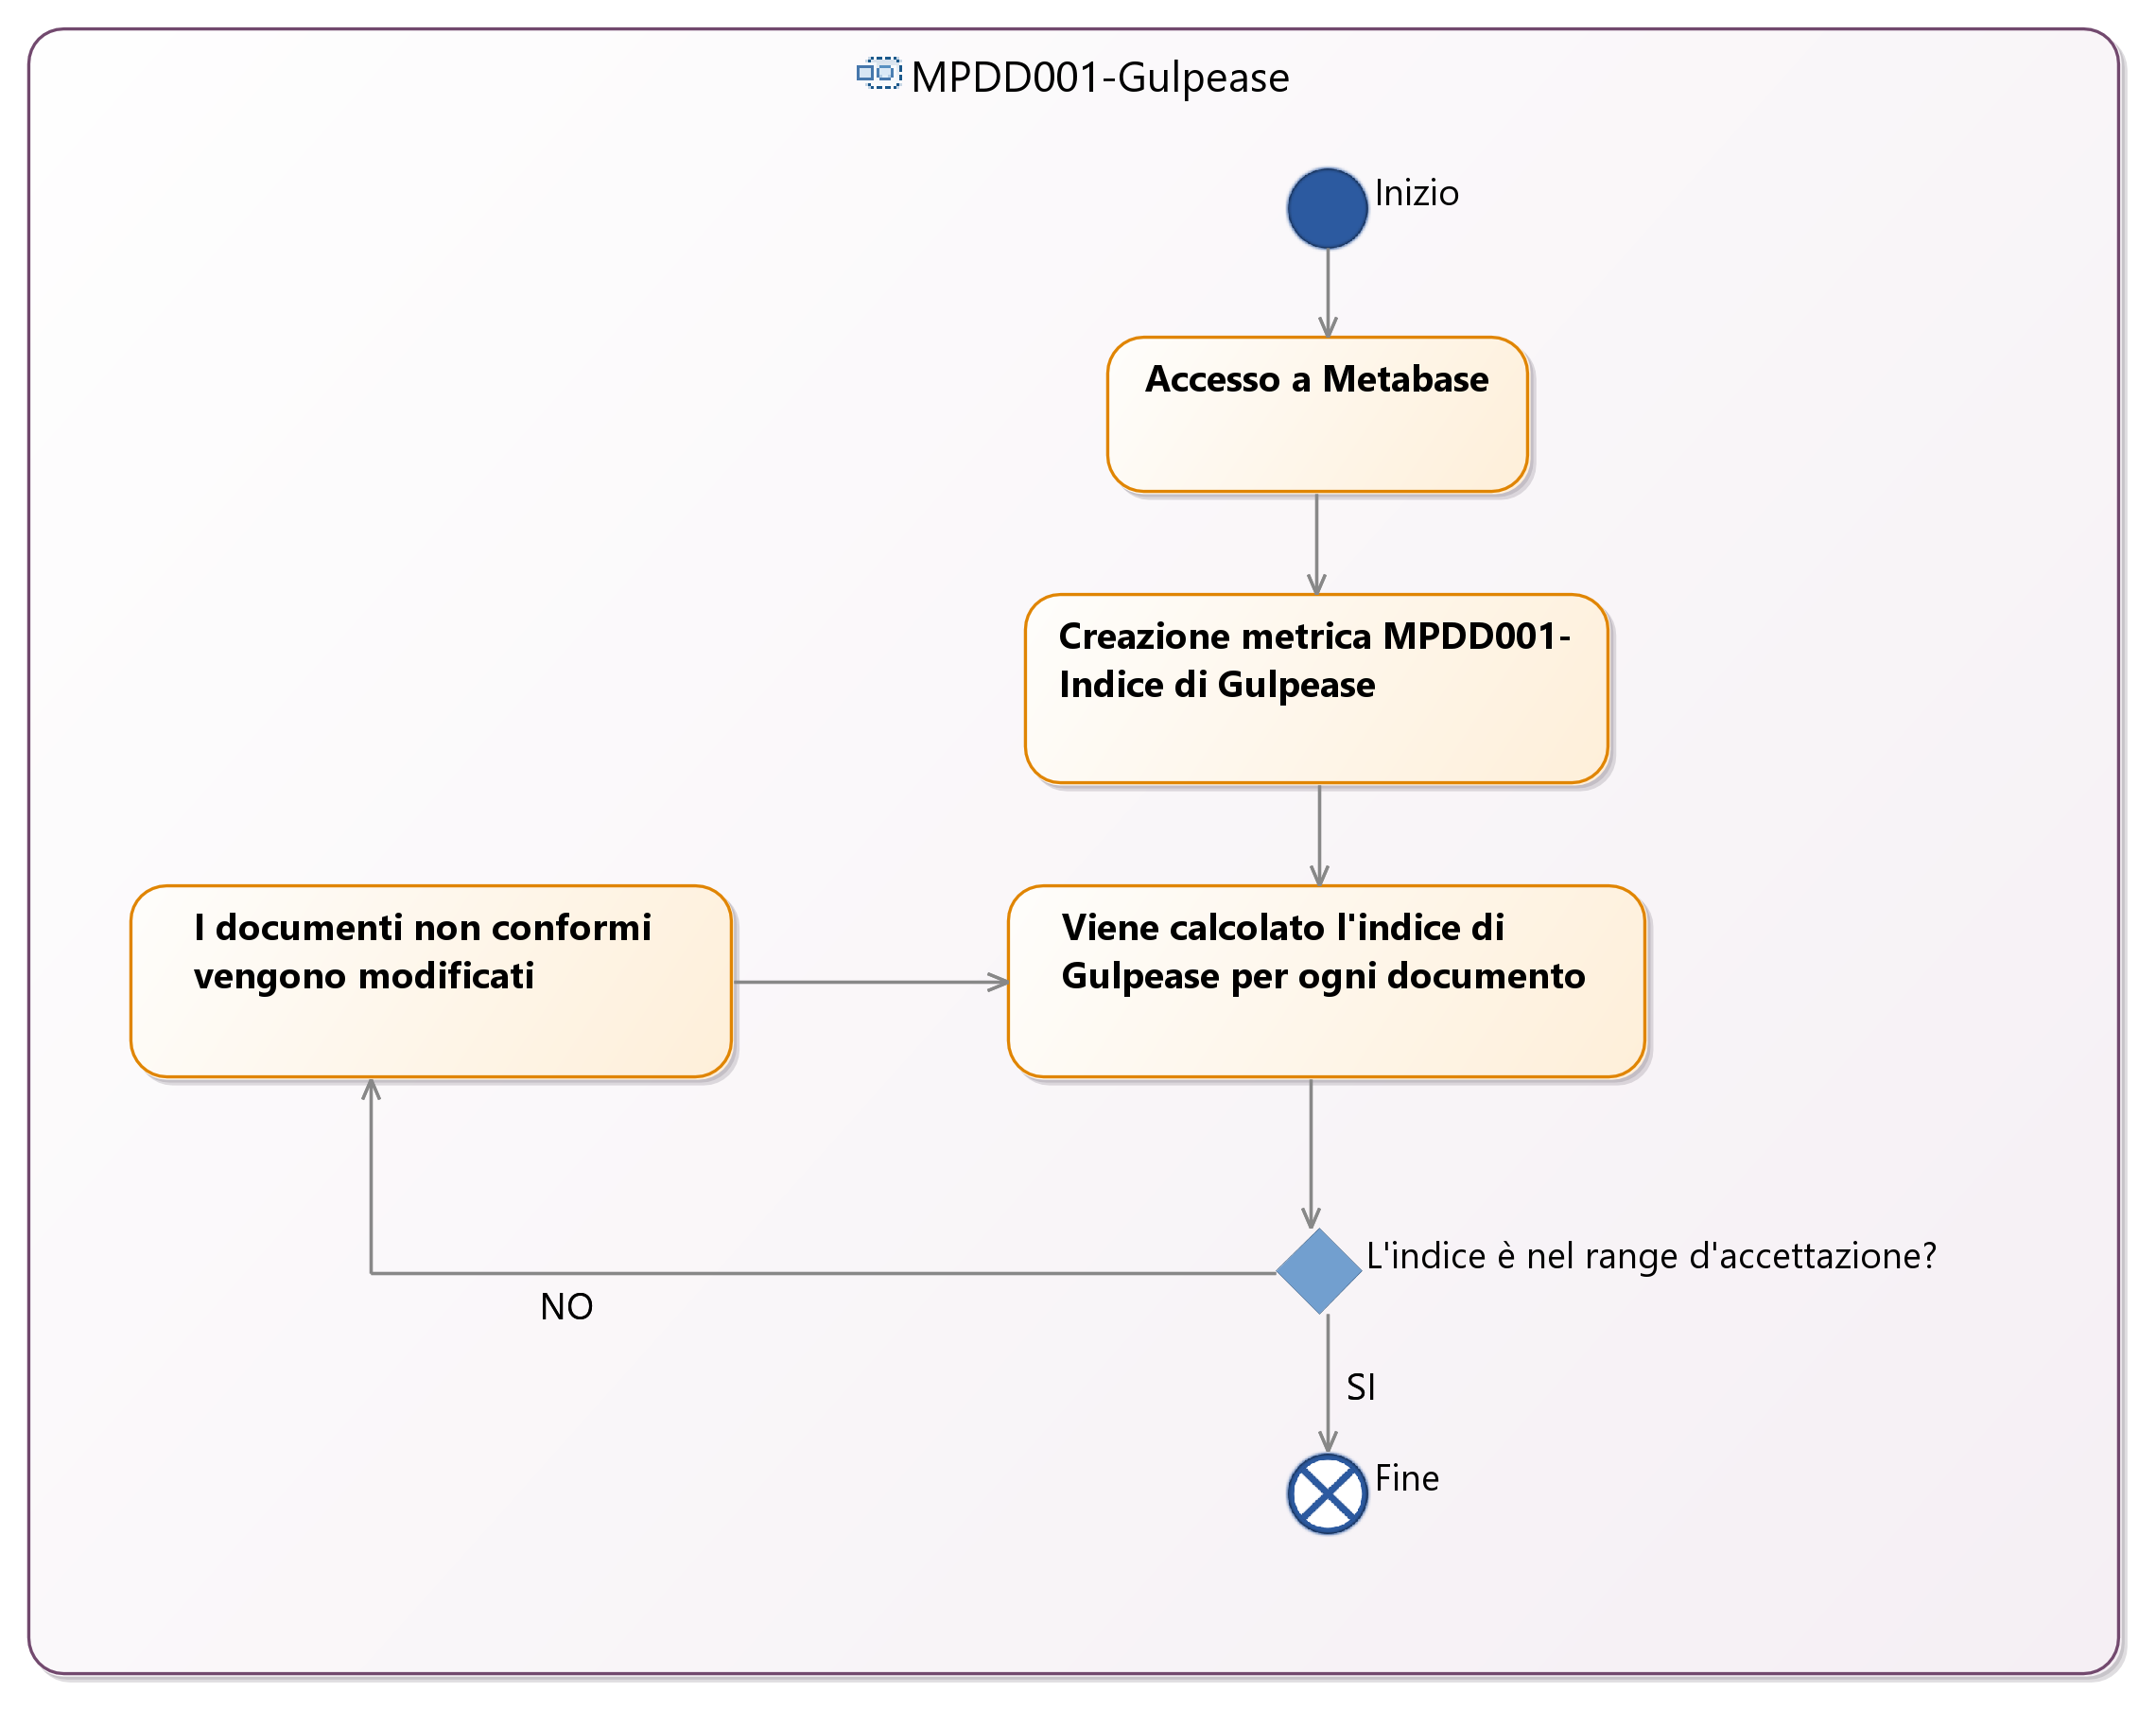
\includegraphics[scale=0.25]{../../common/images/MetricaGulpease}
	 % calcolata tramite lo script "gulpease.py" citato nella sottosezione \textbf{Strumenti di supporto alla documentazione}.\\
	%L'implementazione di ulteriori metriche tramite procedure verrà studiato con l'avanzare del progetto.
	
	\section{Procedure di controllo di qualità di processo}
	La qualità dei processi verrà garantita dall'applicazione del metodo \citGloss{PDCA}, descritto dell'appendice A. Grazie a questo metodo sarà possibile ottenere un miglioramento continuo della qualità di tutti i processi, inclusa la \citGloss{verifica}, e come diretta conseguenza si otterrà il miglioramento dei prodotti risultanti.\\Per ottenere qualità dei processi, bisogna:
	\begin{itemize}
		\item \textbf{Definire il processo}: Affinché sia controllabile;
		\item \textbf{Controllare il processo}: In funzione dell'ottenimento di efficacia, efficienza ed esperienza;
		\item \textbf{Usare strumenti di valutazione}: SPICE e \citGloss{PDCA}.
	\end{itemize}
	
	\section{Processi}
	\subsection{PROC001 - Pianificazione di progetto, impostazione e controllo di processi}
	Il macro-processo ha lo scopo di produrre dei piani di sviluppo per il progetto, comprendenti la scelta del modello di ciclo di vita del prodotto, descrizioni delle attività e dei compiti da svolgere, pianificazione temporale del lavoro e dei costi da sostenere, allocazione di compiti e responsabilità e misurazioni per rilevare lo stato del progetto rispetto alle pianificazioni prodotte.
	
	\subsubsection{Obbiettivi}
	Lo sviluppo del progetto dovrà porre particolare attenzione a rispettare dei particolari obbiettivi:
	\begin{itemize}
		\item \textbf{Budget:} Utilizzando le metriche descritte nella sezione seguente, si deve tenere sempre controllato l'utilizzo del budget, al fine di non avere scarti eccessivi con il costo preventivato;
		\item \textbf{Task:} Porre attenzione alla pianificazione dei task e al loro completamento, assicurandosi che seguano la metodologia del miglioramento continuo, affinché tutti i compiti ne traggano vantaggio;
		\item \textbf{Educazione personale:} Avere accortezza che ogni membro del gruppo abbia un livello di preparazione adatto all'esecuzione dei task assegnati, al fine di evitare ritardi sul calendario;
		\item \textbf{Calendario:} Assicurare una pianificazione adatta ai compiti da svolgere, per evitare scostamenti dal budget preventivato;
		\item \textbf{Standard:} Definire standard di processo ogni qualvolta sia possibile, per facilitare il lavoro in gruppo e favorire un incremento continuo.
	\end{itemize}
	
	\subsubsection{Strategie}
	Ogni eventuale valore negativo a livello di Schedule o Budget Variance rilevato sarà compensato con la revisione delle attività da svolgere e i \citGloss{requisiti} da ottenere, per valutare se nei tempi di calendario stabiliti la pianificazione sia corretta o se sia necessario rivedere la programmazione.\\
	Il controllo verrà favorito con strumenti come \citGloss{Asana} e i diagrammi di \citGloss{Gantt} in modo tale da verificare l'andamento del progetto, per avere sempre una visione chiara e quantificabile del lavoro in corso affinché il lavoro non subisca ritardi.\\
	Saranno sempre presenti delle finestre di \citGloss{Slack} per evitare sovrapposizioni di task dovute a eventuali ritardi o imprevisti. 
	
	\subsubsection{Metriche} 
	\paragraph{MPS001 Schedule Variance (SV)}
	Indica se si è in linea, in anticipo o in ritardo, rispetto alla schedulazione delle attività di progetto pianificate nella \citGloss{baseline}.\\
	È un indicatore di efficacia soprattutto nei confronti del Cliente. \\
	Se il valore SV ottenuto è positivo significa che il progetto sta procedendo con una maggiore velocità rispetto a quanto pianificato, viceversa se negativo.\\
	\textbf{Misurazione:}
	\begin{center}
		$ SV = BCWP – BCWS $
	\end{center}
	Dove: \begin{itemize}
		\item \textbf{BCWP (Budgeted Cost of Work Performed)}: \`{E} il valore (in giorni o Euro) delle attività realizzate alla data corrente.
		Rappresenta il valore prodotto dal progetto ossia la somma di tutte le parti completate e di tutte le porzioni completate delle parti ancora da terminare.
		\item \textbf{BCWS (Budgeted Cost of Work Scheduled)}: \`{E} il costo pianificato (in giorni o Euro) per realizzare le attività di progetto alla data corrente.
	\end{itemize}
	
	
	\paragraph{MPS002 Budget Variance (BV)}
	Indica se alla data corrente si è speso di più o di meno rispetto a quanto previsto a budget alla data corrente.\\
	È un indicatore che ha un valore unicamente contabile e finanziario.\\
	Se il valore BV ottenuto è positivo significa che il progetto sta spendendo il proprio budget con minor velocità di quanto pianificato, viceversa se negativo.\\
	\textbf{Misurazione:}
	\begin{center}
		$ BV = BCWS – ACWP $
	\end{center}
	Dove: \begin{itemize}
		\item \textbf{BCWS (Budgeted Cost of Work Scheduled)}: \`{E} il costo pianificato (in giorni o Euro) per realizzare le attività di progetto alla data corrente;
		\item \textbf{ACWP (Actual Cost of Work Performed)}: \`{E} il costo effettivamente sostenuto (in giorni o Euro) alla data corrente.
	\end{itemize}
	
	\subsection{PROC002 - Verifica software}
	Il processo punta a verificare se qualsiasi elemento del sistema soddisfa completamente i \citGloss{requisiti} ad esso assegnati.
	\subsubsection{Obiettivi}
	Per poter definire delle \citGloss{baseline} per lo sviluppo del software, è necessario che il codice venga sempre verificato:
	\begin{itemize}
		\item \textbf{Commenti al codice:} Ogni unità di codice dovrà essere sufficientemente commentata affinché sia ritenuta verificabile;
		\item \textbf{Prevenzione di bug:} Accertarsi per quanto possibile che ogni unità di codice non sia affetta da bug prima dell'utilizzo.
	\end{itemize}
	\subsubsection{Strategie}
	
	Per prevenire bug e vulnerabilità al codice si utilizzano strumenti come Sonarlint e Sonarqube al fine di evitare la propagazione di errori ed avere una panoramica sullo stato generale del codice prodotto.\\
	Si utilizzeranno delle metriche di Code Coverage per avere consapevolezza della quantità di codice testato e poter agire di conseguenza.
	
	\subsubsection{Metriche}
	\paragraph{Code Coverage}
	Per poter avere una misura di codice testato e verificato si adoreranno determinati coverage criteria:
	
	\begin{itemize}
		\item \textlink{MPS003TAB}{MPS003}{\textbf{MPS003 Function coverage:}} Verificare che ogni funzione sia stata chiamata;
		\item \textlink{MPS004TAB}{MPS004}{\textbf{MPS004 Statement coverage:}} Verificare che ogni statement del codice sia stato eseguito; 
		\item \textlink{MPS005TAB}{MPS004}{\textbf{MPS005 \citGloss{Branch} coverage:}} Verificare se tutti i possibili \citGloss{branch} (derivanti da if e case statement) sono stati eseguiti;
		\item \textlink{MPS006TAB}{MPS006}{\textbf{MPS006 Condition coverage:}} Verificare se ogni condizione booleana è stata valutata sia nella condizione true che false. 
		
	\end{itemize}
	\textbf{Misurazione:}
	Vengono calcolate in percentuale sulla quantità di codice testato e verificato oltre che sul totale delle linee di codice scritte, tramite tool automatici come IstanbulJS\footnote{\nURI{https://istanbul.js.org/}}.
	
	\subsection{PROC003 - Gestione rischi}
	Il processo mira ad identificare nuovi rischi e a monitorare e ridurre la possibilità dell'insorgere di questi durante l'attività di progetto.
	\subsubsection{Obiettivi:}
	\begin{itemize}
		\item \textbf{Individurare rischi Fase:} Ad ogni nuova fase del progetto verranno analizzati possibili rischi, cercando delle soluzioni automatiche per diminuire l'occorrenza di questi;
		\item \textbf{Analisi:} I rischi saranno gestiti con una prima analisi che dovrà fornire uno strumento o procedura automatica per ridurre o prevenire le cause scatenanti di questo rischio.
	\end{itemize}
	\subsubsection{Strategie}
	Nel caso dovessero sorgere troppi rischi il gruppo dovrà sospendere i lavori eliminando il maggior numero di questi per permettere la prosecuzione del lavoro.
	Viene utilizzato StatusTicker\footnote{\nURI{https://swe353.statusticker.com}} per avere un cruscotto informativo sullo status dei servizi esterni utilizzati.
	
	\subsubsection{Metriche}
	\paragraph{MPS007 Indisponibilità servizi esterni:} numero totale di giorni in cui siano stati offline o bloccati servizi usati.\\
	\textbf{Misurazione:}
	Indice numerico incrementato partendo da zero per ogni giorno in cui i servizi utilizzati dal gruppo siano risultati totalmente offline per la maggior parte del giorno, tramite controllo su \nURI{statusticker.com}.
	
	\paragraph{MPS008 Rischi non previsti:} indice numerico indica la quantità di rischi esterni a quelli presenti nell'attività di analisi dei rischi rilevati nella corrente fase di progetto. \\
	\textbf{Misurazione:}
	Indice numerico incrementato partendo da 0 per ogni rischio che si manifesta senza essere stato individuato precedentemente nella lista di rischi.
	Viene resettato all'inizio di ogni nuova fase di progetto.
	
	\subsection{PROC004 - Gestione Test}	
	Per garantire una gestione efficacie dell'analisi dinamica è necessario stabilire delle misurazioni sull'esecuzione di essa.
	Le misure elencate qui sotto sono consigliate dal blog di una azienda che produce prodotti di riferimento per la gestione dei test, le informazioni possono essere trovate nei riferimenti informativi.
	\subsubsection{Per tutti i test}
	\paragraph{Tracciamento}
	Questa categoria di misurazioni si occupa di tenere traccia delle esecuzioni dei test e relativi successi fallimenti tramite le seguenti metriche:
	\begin{itemize}
		\item \textbf{MTSA001 Percentuale di test case passati:} indica la percentuale di test case passati, molto utile per capire a che punto si è nella fase di sviluppo della componente. La sua formula di misurazione è la seguente:
		\[PPT=\dfrac{PT}{ET}*100\]
		Dove PT indica il numero di test passati e ET il numero di test eseguiti;
		\item \textbf{MTSA002 Percentuale di test case falliti:} complementare della misurazione precedente. La sua formula di misurazione è la seguente:
		\[PFT=\dfrac{FT}{ET}*100\]
		Dove FT indica il numero di test falliti ed ET quello di test eseguiti;
		\item \textbf{MTSA003 Tempo medio del team di sviluppo per la risoluzione di errori:} indica la quantità di tempo medio utilizzato per risolvere un bug dal team di sviluppo, utile per capire l'impatto medio dell'introduzione di un bug sui tempi di sviluppo. La sua formula di misurazione è la seguente:
		\[TMRE=\dfrac{TTBF}{TB}\]
		Dove TTBF indica il tempo totale speso per la correzione dei difetti (sviluppo e test) e TB il numero totale di bug trovati.
	\end{itemize}
	
	\paragraph{Efficienza}
	Questa categoria di misurazioni mira a valutare l'efficienza di scrittura ed esecuzione dei test.
	\begin{itemize}
		\item \textbf{MTSA004 Efficienza della progettazione dei test:} Indica il tempo medio per la scrittura di un test, un numero troppo elevato potrebbe indicare che si stanno progettando test troppo complessi o che si sta cercando di testare parti del codice superflue. La sua formula di misurazione è la seguente:
		\[TDE=\dfrac{NTP}{TST}\]
		Dove NTP indica il numero totale di test progettati e TST il tempo per la loro stesura.
		\begin{comment}
		\item \textlink{MTSA005TAB}{MTSA005}{\textbf{MTSA005 Tempo medio per il testing dei bug fix:}} Indica la quantità di tempo medio per testare la risoluzione di un difetto, utile per avere un'idea dell'impatto del testing sull'implementazione di una modifica
		\[TTCD=\dfrac{BFTT}{NDT}\]
		Dove BFTT indica il tempo usato per testare le la correzione dei difetti e NDT il numero di difetti trovati.
		\end{comment}
	\end{itemize}
	\paragraph{Efficacia}
	Questa categoria di misurazioni mira a valutare l'efficacia dell'esecuzione dei test.
	\begin{itemize}
		\item \textbf{MTSA005 Contenimento dei difetti:} Indica il rapporto percentuale tra i bug trovati durante i test e i bug trovati durante l'utilizzo del prodotto. Un numero troppo basso di questo indice suggerisce una scarsa progettazione dei test, richiedendo un intervento di analisi da parte del team di sviluppo. La sua formula di misurazione è la seguente:
		\[CD=\dfrac{DTT}{TNDT}*100\]
		Dove DTT indica il numero di difetti trovati durante l'esecuzione dei test, e TNDT la somma dei difetti trovati nei test e quelli trovati durante l'utilizzo del prodotto.
	\end{itemize}
	
	\subsubsection{Per i test ad alto livello}
	\paragraph{Tracciamento}
	Questa categoria di misurazioni mira a tenere traccia delle gestioni dei bug trovati.
	\begin{itemize}
		\item \textbf{MTSH001 Percentuale di difetti sistemati:} indica la percentuale di difetti sistemati sul totale dei difetti rilevati, utile per avere una panoramica dei bug da risolvere: un numero troppo basso potrebbe costringere il team a fermare lo sviluppo di nuove funzionalità per concentrarsi sulla correzione delle parti già esistenti. La sua formula di misurazione è la seguente:
		\[PDS=\dfrac{DS}{DR}*100\]
		Dove DS indica i difetti sistemati mentre DR quelli segnalati.	
	\end{itemize}
	\paragraph{Copertura}
	Questa categoria di misurazioni si occupa di tenere traccia dell'esecuzione dei test e della copertura che questi hanno sui \citGloss{requisiti}.
	\begin{itemize}
		\item \textbf{MTSH002 Copertura dei test eseguiti:} Indica la percentuale di test già eseguiti sul totale di test da eseguire, utile per monitorare il lavoro del team dei verificatori. La sua formula di misurazione è la seguente:
		\[CTE=\dfrac{TE}{TT}*100\]
		Dove TE indica i test eseguiti e TT il numero di test totali;
		\item \textbf{MTSH003 Copertura dei requisiti:} Indica la percentuale di requisiti coperti dai test sui requisiti totali, utile per capire quante parti del prodotto finale hanno un test associato, non da indicazioni sullo stato di avanzamento del soddisfacimento del requisito. La sua formula di misurazione è la seguente:
		\[CR=\dfrac{RC}{RT}*100\]
		Dove RC indica il numero di \citGloss{requisiti} coperti mentre RT quelli totali;
		\item \textbf{MTSH004 Difetti per requisito:} Indica il numero di difetti trovati nel test del requisito, da informazioni sullo stato di soddisfacimento del requisito: se ha 0 difetti, vuol dire che il requisito è stato trovato e considerato senza errori, quindi soddisfatto.
		Non essendo calcolabile, la misurazione si mostra come una tabella avente nella prima colonna il nome del requisito, e nella seconda i difetti ad esso associati.
	\end{itemize}
	\begin{comment}
	\paragraph{Efficacia dei cambiamenti}
	\begin{itemize}
	\item \textlink{MTSH005TAB}{MTSH005}{\textbf{MTSH005 Tasso di iniezione dei difetti:}} Indica il tasso di errori attribuibili all'introduzione di una modifica, la conoscenza di questo numero aiuta a stimare il tempo medio per la scoperta e correzione di errori introdotti dalle modifiche, aiutando la stima dei costi per l'introduzione di nuove funzionalità
	\[TID=\dfrac{NM}{NDM}\]
	Dove NM indica il numero di modifiche e NDM i difetti attribuibili ad esse.
	\end{itemize}
	\end{comment}
	
	\section{Prodotti}
	\subsection{Qualità dei documenti}
	I documenti prodotti dal gruppo \gruppo dovranno essere leggibili, comprensibili e corretti dal punto di vista ortografico, sintattico, logico e semantico.
	\subsubsection{Obiettivi di qualità: comprensione}
	\begin{itemize}
		\item \textbf{Leggibilità:} i documenti prodotti dovranno essere leggibili e comprensibili a persone con licenza di istruzione media;
		\item \textbf{Correttezza ortografica:} i documenti prodotti non dovranno contenere errori ortografici.
	\end{itemize}
	
	\subsubsection{Metriche}
	\begin{itemize}
		\item \textbf{MPDD001 Indice di Gulpease:} è l'indice di leggibilità tarato sulla lingua italiana. Considera due variabili linguistiche: la lunghezza della parola e la lunghezza della frase rispetto al numero di lettere. La formulata per il suo calcolo è la seguente:
		\[IG=89+\dfrac{300*N_F-10*N_L}{N_P}\] Dove $ N_F $ è il numero delle frasi, $ N_L $ il numero delle lettere e $ N_P $ il numero delle parole. Il risultato $I$ è un numero compreso tra 0 e 100. In generale risulta che i testi con indice inferiore a:
		\begin{itemize}
			\item 80 sono difficili da leggere per chi ha una licenza elementare;
			\item 60 sono difficili da leggere per chi ha una licenza media;
			\item 40 sono difficili da leggere per chi ha un diploma superiore.
		\end{itemize}	
		\item \textbf{MPDD002 Formula di Flesch:} è una formula che serve per misurare la leggibilità di un testo in inglese:
		\[F=206,835-(0,846*S)-(1,015*P)\] Dove $ S $ è il numero delle sillabe, calcolato su un campione di 100 parole e $ P $ è il numero medio di parole per frase.
		La leggibilità è alta se $F$ è superiore a 60, media se fra 50 e 60, bassa sotto a 50;
		\item \textbf{MPDD003 Errori ortografici:} gli errori ortografici possono essere identificati tramite lo strumento \textquoteleft Controllo ortografico\textquoteright\ presente in \citGloss{TexStudio}. Sarà poi compito del Verificatore correggerli.  	
	\end{itemize}
	
	\subsection{Qualità del software}
	\subsubsection{Funzionalità:} Rappresenta la capacità del prodotto di fornire tutte le funzionalità che sono state individuate attraverso l'\adr.	
	\paragraph{Obiettivi qualità}
	Il gruppo \gruppo si impegnerà per perseguire:
	\begin{itemize}
		\item \textbf{Adeguatezza}: le funzionalità fornite siano conformi rispetto le aspettative;
		\item \textbf{Accuratezza}: il prodotto fornisca i risultati attesi, con il livello di dettaglio richiesto. 
	\end{itemize}	
	\paragraph{Metriche}
	\begin{itemize}
		\item \textbf{MPDS001 Copertura requisiti obbligatori:} indica la percentuale dei requisiti obbligatori coperti dall'implementazione. La sua formula di misurazione è la seguente: \[CRO=(\frac{N_{ROS}}{N_{RO}})*100\] Dove $ N_{ROS} $ è il numero di requisiti obbligatori soddisfatti e $ N_{RO} $ è il numero totale dei requisiti obbligatori;
		\item \textbf{MPDS002 Copertura requisiti accettati:} indica la percentuale dei requisiti desiderabili e facoltativi coperti dall'implementazione. La sua formula di misurazione è la seguente: \[CRA=(\frac{N_{RAS}}{N_{RA}})*100\] Dove $ N_{RAS} $ è il numero di requisiti accettati soddisfatti e $ N_{RA } $ è il numero totale dei requisiti accettati;
		\item \textbf{MPDS003 Accuratezza rispetto alle attese:} indica la percentuale di risultati concordi alle attese. La sua formula di misurazione è la seguente: \[ARA=(1-\frac{N_{TD}}{N_{TE}})*100\] Dove $ N_{TD} $ è il numero di test che producono risultati discordi alle attese e $ N_{TE} $ è il numero di test-case eseguiti.
	\end{itemize}
	
	\subsubsection{Affidabilità}
	Rappresenta la capacità del prodotto software di svolgere correttamente le sue funzioni durante il suo utilizzo, anche in caso in cui si presentino situazioni anomale.
	\paragraph{Obiettivi di qualità}
	L'esecuzione del prodotto dovrà presentare le seguenti caratteristiche:
	\begin{itemize}
		\item \textbf{Maturità:} evitare che si verifichino malfunzionamenti, operazioni illegali e \citGloss{failure} in seguito a \citGloss{fault};
		\item \textbf{Tolleranza agli errori:} nel caso in cui si presentino degli \citGloss{errori}, dovuti a guasti o ad un uso scorretto dell'applicativo, questi devo essere gestiti in modo da mantenere alto il livello di prestazioni.
	\end{itemize}
	\paragraph{Metriche}
	\begin{itemize}
		\item \textlink{MPDS004TAB}{MPDS004}{\textbf{MPDS004 Densità di failure:}} indica la percentuale di testing che si sono concluse in failure. La sua formula di misurazione è la seguente: \[DF=(\frac{N_{FR}}{N_{TE}})*100\] Dove $ N_{FR} $ è il numero di failure rilevati durante l'attività di testing e $ N_{TE} $ è il numero di test-case eseguiti;
		\item \textlink{MPDS005TAB}{MPDS005}{\textbf{MPDS005 Blocco di operazioni non corrette:}} indica la percentuale di funzionalità in grado di gestire correttamente i fault che potrebbero verificarsi. La sua formula di misurazione è la seguente: \[BNC=(\frac{N_{FE}}{N_{ON}})*100\] Dove $ N_{FE} $ è il numero di failure evitati durante i test effettuati e $ N_{ON} $ è il numero di test-case eseguiti che prevedono l'esecuzione di operazioni non corrette, causa di possibili failure.
	\end{itemize}
	\subsubsection{Usabilità}
	Rappresenta la capacità del prodotto di essere facilmente comprensibile ed attraente in ogni sua parte per qualsiasi utente che lo andrà ad utilizzare.
	\paragraph{Obiettivi di qualità}
	Il prodotto dovrà puntare ai seguenti obiettivi di usabilità:
	\begin{itemize}
		\item \textbf{Comprensibilità:} l'utente deve essere in grado di riconoscere le funzionalità offerte dal software e deve comprendere le modalità di utilizzo per raggiungere i risultati attesi;
		\item \textbf{Apprendibilità:} deve essere data la possibilità all'utente di imparare ad utilizzare l'applicazione senza troppo impegno;
		\item \textbf{Operabilità:} le funzioni presenti devono essere coerenti con le aspettative dell'utente;
		\item \textbf{Attrattiva:} il software deve essere piacevole per chi ne fa uso.
	\end{itemize}
	\paragraph{Metriche}
	\begin{itemize}
		\item \textbf{MPDS006 Comprensibilità delle funzioni offerte:} indica la percentuale di operazioni comprese in modo immediato dall'utente, senza la consultazione del manuale. La sua formula di misurazione è la seguente: \[CFC=(\frac{N_{FC}}{N_{FO}})*100\] Dove $ N_{FC} $ è il numero di funzionalità comprese in modo immediato dall'utente durante l'attività di testing del prodotto e $ N_{FO} $ è il numero di funzionalità offerte dal sistema;
		\item \textbf{MPDS007 Facilità di apprendimento delle funzionalità:} indica il tempo medio impiegato dall'utente nell'imparare ad usare correttamente una data funzionalità. Si misura tramite un indicatore numerico che indica i minuti impiegati da un utente per apprendere il funzionamento di una certa funzionalità;
		\item \textbf{MPDS008 Consistenza operazionale in uso:} indica la percentuale di messaggi e funzionalità offerte all'utente che rispettano le sue aspettative riguardo al comportamento del software. La sua formula di misurazione è la seguente: \[COU=(\frac{N_{MFU}}{N_{MFO}})*100\] Dove $ N_{MFU} $ è il numero di messaggi e funzionalità che non rispettano le aspettative dell'utente e $ N_{MFO} $ è il numero di messaggi e funzionalità offerte dal sistema.	
	\end{itemize}	
	\paragraph{Misurazione}
	Queste metriche di usabilità misurate tramite sessioni di prova con utenti esterni per dar modo di ottenere feedback reali e misurazioni attendibili.\\ Ogni sessione sarò registrata per uso interno al gruppo tramite screen recorder e microfono, gli utenti sarannò istruiti sul cercare e/o utilizzare una serie di funzionalità tracciate da un Verificatore.
	Combinando le misurazioni effettuate si determineranno i valori per le metriche sopra descritte.
	
	\subsubsection{Efficienza}
	Rappresenta la capacità di eseguire le funzionalità offerte dal software nel minor tempo possibile utilizzando al tempo stesso il minor numero di risorse disponibili.
	\paragraph{Obiettivi di qualità}
	Il prodotto dovrà essere efficiente, in particolare:
	\begin{itemize}
		\item \textbf{Comportamento rispetto al tempo:} per svolgere le sue funzioni il software deve fornire adeguati tempi di risposta ed elaborazione;
		\item \textbf{Utilizzo delle risorse:} il software quando esegue le sue funzionalità deve utilizzare un appropriato numero e tipo di risorse.
	\end{itemize}
	\paragraph{Metriche}
	\begin{itemize}
		\item \textbf{MPDS009 Tempo di risposta:} indica il tempo medio che intercorre fra la richiesta software di una determinata funzionalità e la restituzione del risultato all'utente. La sua formula di misurazione è la seguente: \[TR=\frac{\sum_{i=1}^n T_i}{n}\] Dove $ T_i $ è il tempo intercorso fra la richiesta $ i $ di una funzionalità ed il comportamento delle operazioni necessarie a restituire un risultato a tale richiesta.	
	\end{itemize}
	\subsubsection{Manutenibilità}
	Rappresenta la capacità del prodotto di essere modificato, tramite correzioni, miglioramenti o adattamenti del software a cambiamenti negli ambienti, nei \citGloss{requisiti} e nelle specifiche funzionali.
	\paragraph{Obiettivi di qualità}
	Le operazioni di manutenzione andranno agevolate il più possibile adottando le seguenti caratteristiche:
	\begin{itemize}
		\item \textbf{Analizzabilità:} il software deve consentire una rapida identificazione delle possibili cause di errori e malfunzionamenti;
		\item \textbf{Modificabilità:} il prodotto originale deve permettere eventuali cambiamenti in alcune sue parti;
		\item \textbf{Stabilità:} non devono insorgere effetti indesiderati in seguito a modifiche effettuate sul software;
		\item \textbf{Testabilità:} il software deve poter essere facilmente testato per valiare le modifiche effettuate.
	\end{itemize}
	\paragraph{Metriche}
	\begin{itemize}
		\item \textbf{MPDS010 Capacità di analisi di failure:} indica la percentuale di modifiche effettuate in risposta a failure che hanno portato all'introduzione di nuove failure in altre componenti del sistema. La sua formula di misurazione è la seguente: \[CAF=(\frac{N_{FI}}{N_{FR}})*100\] Dove $ N_{FI} $ è il numero di failure delle quali sono state individuate le cause e $ N_{FR} $ è il numero di failure rilevate;
		\item \textbf{MPDS011 Impatto delle modifiche:} indica la percentuale di modifiche effettuate in risposta a failure che hanno portato all'introduzione di nuove failure in altre componenti del sistema. La sua formula di misurazione è la seguente: \[IM=(\frac{N_{FRF}}{N_{FR}})*100\] Dove $ N_{FRF} $ è il numero di failure risolte con l'introduzione di nuove failure e $ N_{FR} $ è il numero di failure risolte.
	\end{itemize}
	\subsubsection{Portabilità}
	Rappresenta la capacità del software di poter essere utilizzato su diversi ambienti.
	\paragraph{Obiettivi di qualità}
	Sarò agevolata la portabilità del prodotto adottando i seguenti obiettivi:
	\begin{itemize}
		\item \textbf{Adattabilità:} il prodotto deve adattarsi a tutti quelli ambienti di lavoro nei quali è stato previsto un suo utilizzo, senza dover apportare modifiche dello stesso;
		\item \textbf{Sostituibilità:} l'applicativo deve poter sostituire un altro software che ha lo stesso scopo e lavora nel medesimo ambiente.
	\end{itemize}
	\paragraph{Metriche}
	\begin{itemize}
		\item \textbf{MPDS012 Versioni dei browser supportate:} indica la percentuale di versioni di browser attualmente supportate, fra quelle individuate dai requisiti. La sua formula di misurazione è la seguente: \[VB=(\frac{N_{VS}}{N_{VI}})*100\] Dove $ N_{VS} $ è il numero di versioni di browser supportate dal prodotto e $ N_{VI} $ è il numero di versioni di browser che devono essere supportate dal prodotto;
		\item \textbf{MPDS013 Inclusione di funzionalità da altri prodotti:} indica la percentuale del software utilizzato in precedenza dall'utente che produce risultati simili a quelli ottenuti dal prodotto in oggetto. La sua formula di misurazione è la seguente: \[IFP=(\frac{N_{FPA}}{N_{FPP}})*100\] Dove $ N_{FPA} $ è il numero di funzionalità del software utilizzato in precedenza dall'utente che produce risultati simili a quelli ottenuti dal prodotto in oggetto e $ N_{FPP} $ è il numero di funzionalità offerte dal software utilizzato in precedenza dall'utente. 
	\end{itemize}
	
	\section{Configurazione}
	
	\subsection{Controllo di versione}
	
	\subsubsection{Descrizione}
	Per le parti versionabili del progetto e per i documenti ufficiali si è scelto l'utilizzo della tecnologia Git.
	La condivisione dei documenti informali e delle parti non versionabili è invece effettuata tramite l'uso di una cartella Google Drive condivisa.
	
	\subsubsection{Struttura delle repository}
	\`{E} stata realizzata solo una \citGloss{repository} durante la fase di RR ossia quella relativa alla documentazione denominata "Documentazione 353", si prevede inoltre di creare ulteriori repository per suddividere lo sviluppo e la codifica dell'applicazione del progetto. \\\\
	I file interni al \citGloss{repository} "Documentazione 353" sono organizzati secondo questa struttura:
	\begin{itemize}
		\item \textbf{Esterni:}
				\begin{itemize}
				\item \textbf{AnalisiDeiRequisiti};
				\item \textbf{Glossario};
				\item \textbf{PianoDiProgetto};
				\item \textbf{PianoDiQualifica};
				\item \textbf{Verbali esterni}.
			\end{itemize}
		\item \textbf{Interni:}
				\begin{itemize}
					\item \textbf{NormeDiProgetto};
					\item \textbf{Glossario};
					\item \textbf{StudioDiFattibilita};
					\item \textbf{Verbali interni}.
				\end{itemize}		
	\end{itemize}	
	All'interno di ogni cartella è stato definito un file \citGloss{LaTeX} principale che assume il nome del documento stesso ed il file diariomodifiche.tex per mantenere traccia delle modifiche effettuate.\\
	Nella root della \citGloss{repository} è stato messo invece un file .sh gestito tramite \citGloss{Travis} CI che controlla automaticamente gli errori in tutti i documenti presenti e compila un log con i risultati ottenuti.
	
	\subsubsection{Ciclo di vita dei branch}
	Per sfruttare il parallelismo nello sviluppo di uno stesso documento sono stati creati appositamente dei \citGloss{branch} denominati con il nome del membro o dei membri del gruppo che devono lavorare su una determinata parte, mentre i documenti baseline saranno invece contenuti nel master \citGloss{branch}.\\
	Il merge col master avviene quindi solamente quando un documento si trova in stato di "Approvato".
	
	\subsubsection{Aggiornamento della repository}
	Per l'aggiornamento della \citGloss{repository} è previsto il seguente sotto processo motivato dalla sezione precedente "ciclo di vita":
	\begin{itemize}
		\item Verificare di trovarsi sul \citGloss{branch} personale con "git branch"(quella selezionata presenta un asterisco *) e in caso di riscontro negativo cambiare branch con "git checkout"
		\item Dare il comando "git pull". Nel caso in cui si verifichino dei conflitti:
		\begin{itemize}
			\item Dare il comando "git stash" per accantonare momentaneamente	le modifiche apportate;
			\item Dare il comando "git pull" per ottenere ed applicare i \citGloss{commit} mancanti;
			\item Dare il comando "git stash apply" per ripristinare le modifiche.
		\end{itemize}
		In questo modo il \citGloss{repository} locale risulta aggiornato rispetto il \citGloss{repository} remoto, mantenendo le modifiche personali apportate;
	
		\item Dare il comando "git add [files]" , che aggiungerà i file modificati e quelli nuovi specificati;
		\item Dare il comando "git commit" e successivamente riassumere le modifiche effettuate, in caso sia utile si può aggiungere un messaggio esteso di descrizione;
		\item Dare il comando "git push" per completare l'operazione e fornire le modifiche agli altri membri del gruppo.
	\end{itemize}
	\subsection{Strumenti}
	\begin{itemize}
		\item \textbf{Client git:} verrano usati due client secondo le preferenze personali di ogni membro del gruppo tra Github Desktop\footnote{\nURI{https://desktop.github.com/}} e GitKraken\footnote{\nURI{https://www.gitkraken.com/}}, gratuito con licenza studenti;
		\item \textbf{Server git:} sarà utilizzato Github\footnote{\nURI{https://github.com/}} per affidabilità ed integrazione con strumenti esterni come \citGloss{Travis} facilitata. Era stato inoltre suggerito dal Referente oltre ad essere già utilizzato dalla maggior parte dei membri del gruppo.
	\end{itemize}

	
	\section{Verifica}
	
	\subsection{Descrizione}
	Un processo fondamentale per il proseguimento e l'evoluzione di un progetto è la \citGloss{verifica} su ogni suo sottoprodotto che porta alla creazione di un singolo componente.\\
	In questa sezione si descriveranno gli strumenti e i metodi che verranno usati per la \citGloss{verifica} del codice e dei documenti durante la loro realizzazione.\\
	Per quanto riguarda questa prima parte di progetto la \citGloss{verifica} si è concentrata essenzialmente su documenti e diagrammi.
	
	\subsection{Analisi statica}
	L'analisi statica è una tecnica di analisi applicabile sia alla documentazione che al codice e permette di effettuare la \citGloss{verifica} di quanto prodotto individuando errori ed anomalie.\\
	Essa può essere svolta in due modi diversi:
		\begin{itemize}
			\item \textbf{Walkthrough:} tecnica applicata quando non si sanno le tipologie di errori o problemi che si stanno cercando e quindi prevede una lettura da cima a fondo del codice o documento per trovare anomalie di qualsiasi tipo.\\
			Viene sempre svolto per la \citGloss{verifica} dei contenuti dei documenti;
						
			\item \textbf{Inspection:} tecnica da applicare quando si ha idea delle possibili problematiche che si stanno cercando e si attua leggendo in modo mirato il documento/codice sulla base di una lista di possibili errori precedentemente stilata.\\
			Viene realizzata tramite la checklist presente sul sito Todo353swe.
		\end{itemize}
	
	\subsection{Analisi dinamica}
	Il processo di analisi dinamica consiste nella realizzazione ed esecuzione di una serie di test sul codice del software di varie tipologie. Questa tecnica non è applicabile per trovare errori nella documentazione.
	
	\subsection{Verifica Diagrammi UML}
	I verificatori devono controllare tutti i diagrammi UML prodotti rispettino lo standard UML e che siano corretti semanticamente.
	
	\subsection{Strumenti}
	\begin{itemize}
		\item \textbf{Software:} verranno usati per la verifica Mocha ed Enzyme per React, Jest per Redux, mentre per i contratti Solidity useremo Mocha e Chai ma verranno attualizzati e confermati per la Technology \citGloss{baseline};
		\item \textbf{Documenti:} per il controllo dei documenti prodotti utilizzeremo le funzionalità di Texstudio assieme a script bash eseguiti automaticamente da \citGloss{Travis} per controllare che non ci siano errori nei file \citGloss{LaTeX}, per assicurarsi che il Glossario non presenti mancanze o duplicati e verificare l'assenza di errori ortografici;
		\item \textbf{Gestione processi e feedback:} è stato scelto di utilizzare il sistema integrato di issues\footnote{\nURI{https://guides.github.com/features/issues/}} presente su \citGloss{GitHub} per permettere un dialogo maggiore per ogni singola issue. 
		\item \textbf{Gestione tasklist:} Todo353swe\footnote{\nURI{https://todo353swe.netlify.com}} semplice sito per gestione tasklist realizzato dai membri del gruppo per utilizzo interno.
		\item \textbf{Analisi dinamica locale:} è stato individuato un plugin per Webstorm SonarLint\footnote{\nURI{https://plugins.jetbrains.com/plugin/7973-sonarlint}} come soluzione iniziale da verificare, per risolvere tutte le necessità di analisi del codice locale. Maggiori dettagli sarannò forniti durante la creazione dei Proof of concept per la Technology \citGloss{baseline}.
		\item \textbf{Analisi dinamica remota:} è stato individuato Sonarqube\footnote{\nURI{https://www.sonarqube.org/}} come soluzione iniziale da accertare, per risolvere tutte le necessità di analisi del codice del gruppo. Maggiori dettagli sarannò introdotti durante la creazione dei Proof of concept per la Technology \citGloss{baseline}.
	\end{itemize}


	\section{Validazione}
	\subsection{Descrizione}
		Il processo di \citGloss{validazione} ha l'obiettivo di verificare che il prodotto sia conforme a quanto pianificato e sia abile nel gestire e minimizzare gli effetti degli errori.
	\subsection{Procedure}
		I passi per compiere l’attività di \citGloss{validazione} sono i seguenti:\\
		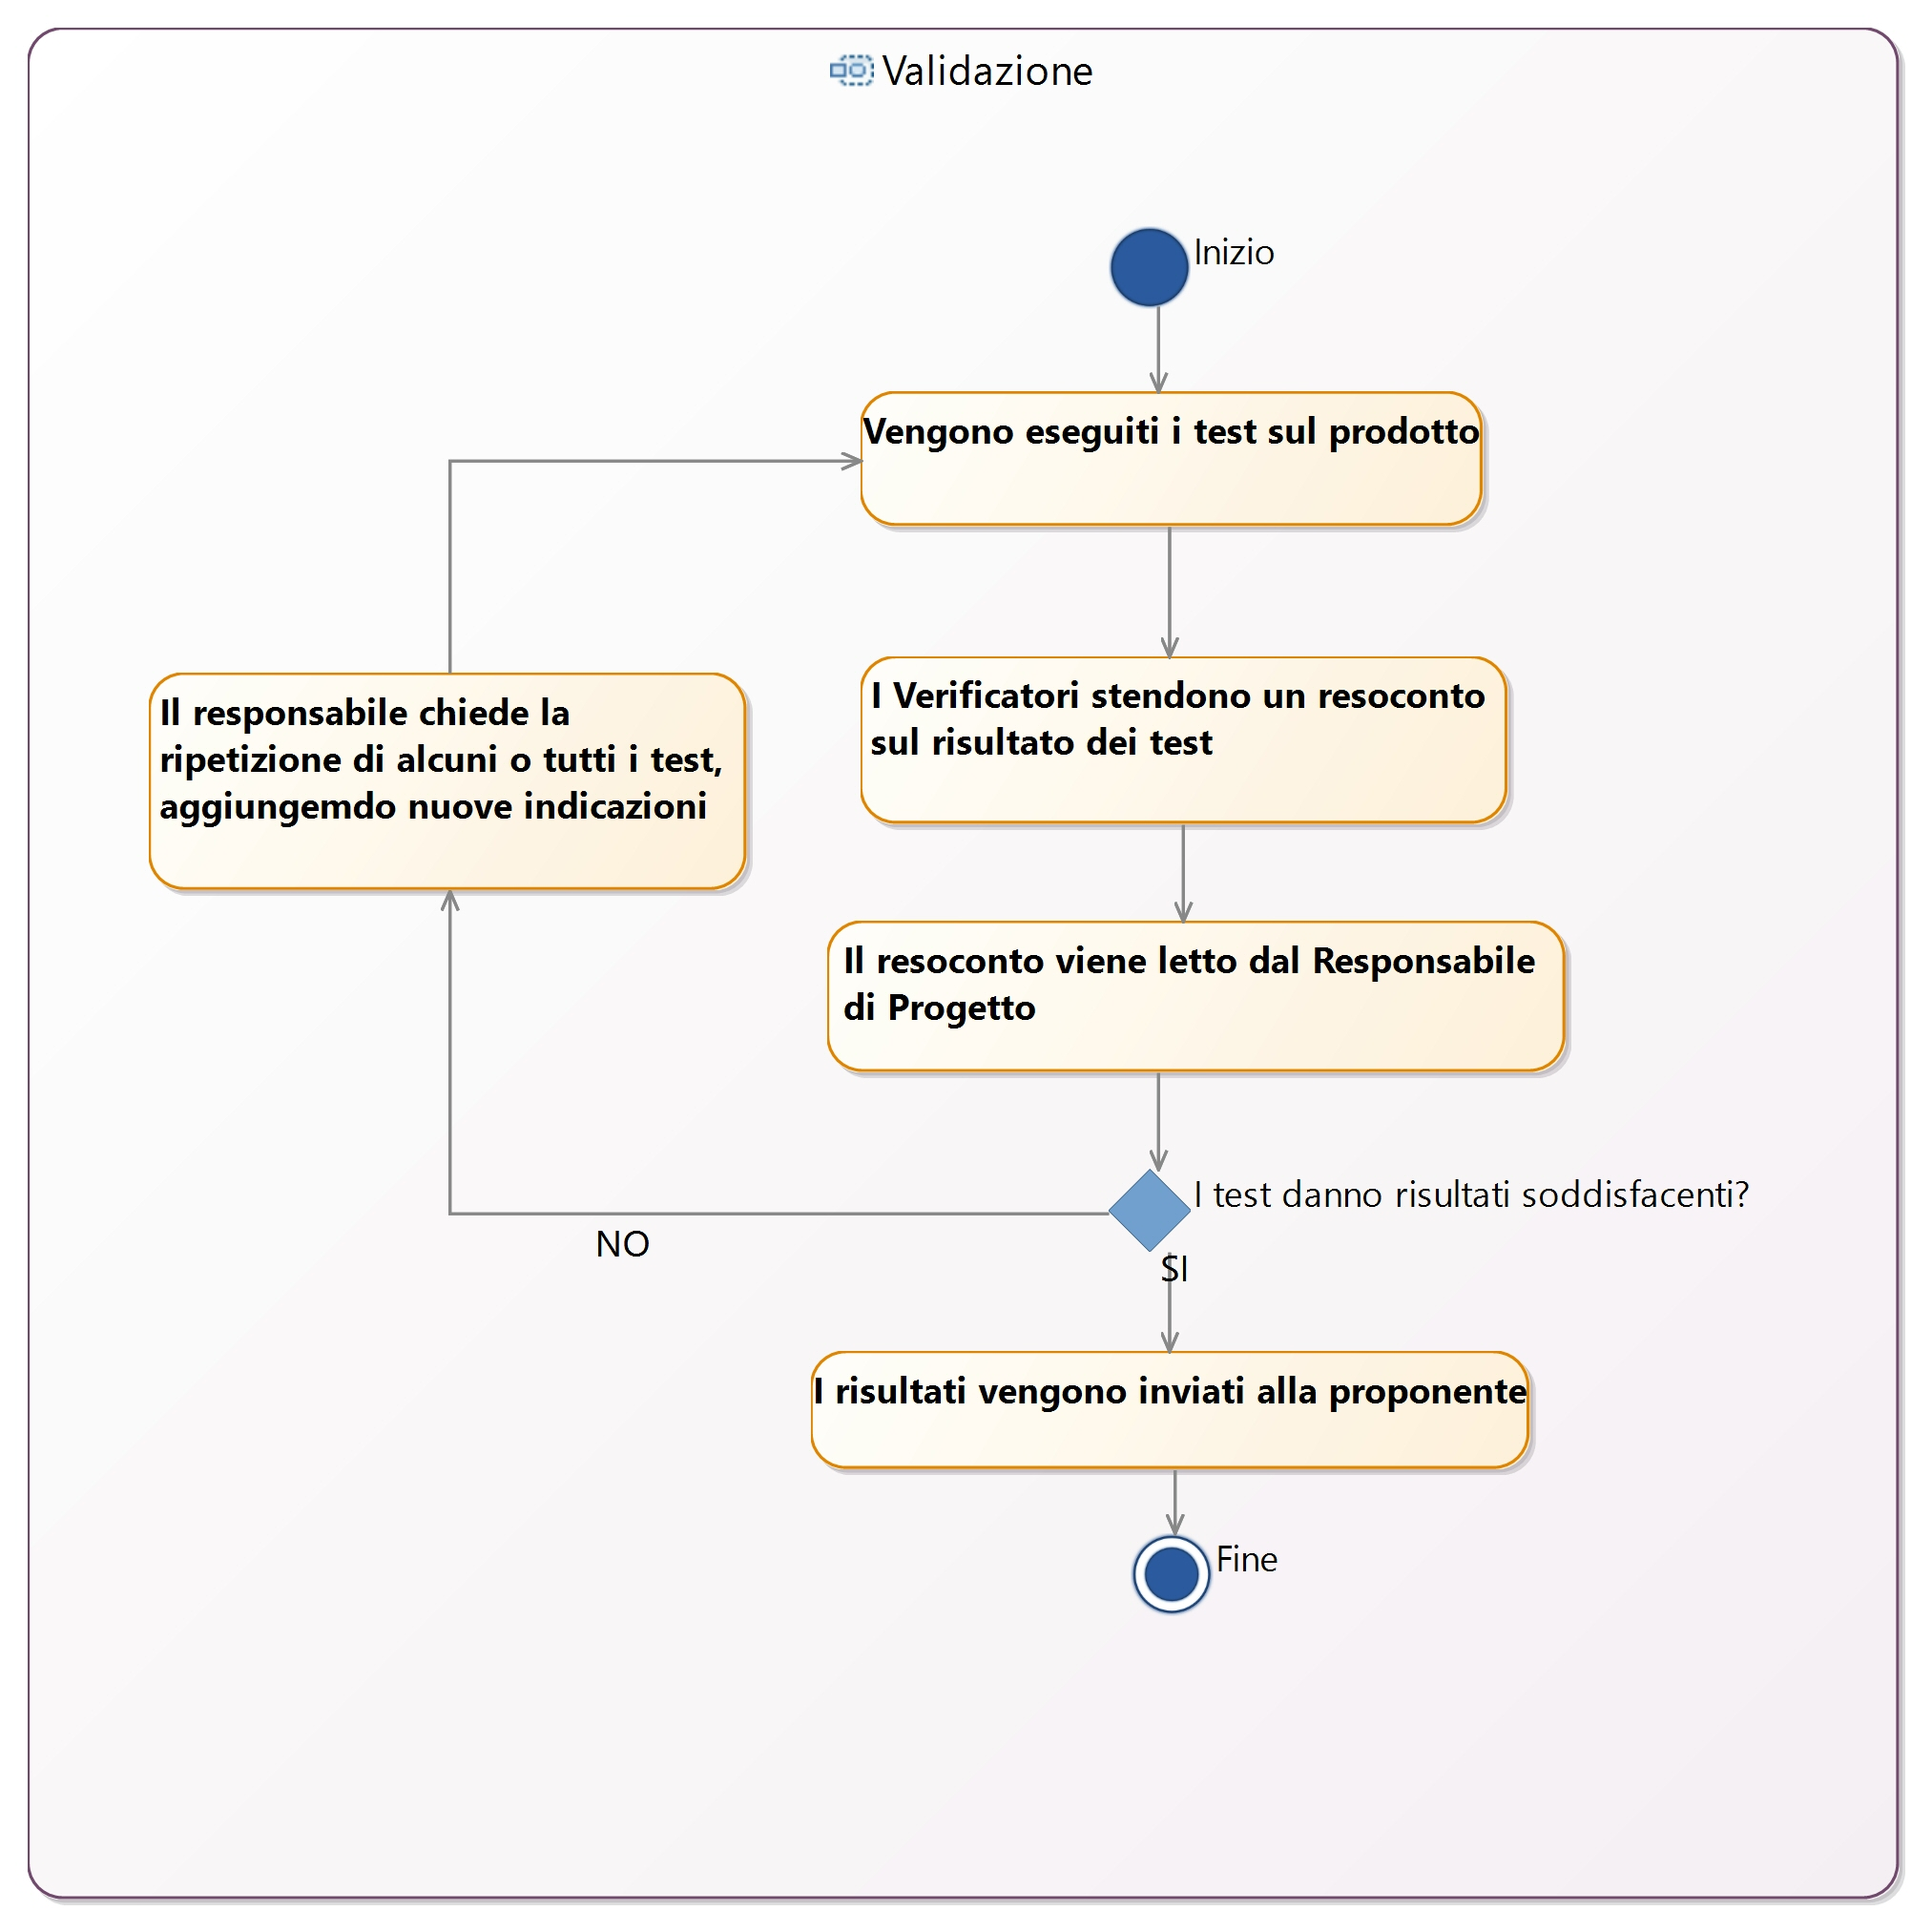
\includegraphics[scale=0.2]{../../common/images/Validation}

	 
	
	
\end{document}